\documentclass{beamer} 
\usetheme{default} 
\setbeamercovered{transparent}

%\useoutertheme{umbcfootline} 
\setbeamertemplate{background canvas}[vertical shading][bottom=red!20,top=yellow!30] 


\usepackage[spanish]{babel}
%\usepackage[latin1]{inputenc}
\usepackage[utf8x]{inputenc}
\usepackage{hyperref}
\usepackage{color}

\title{Cuadros de dialogos}

\author{Manuel J. Molino Milla \and Luis Molina Garzón}

\date{\today} %

\institute{IES Virgen del Carmen \and Departamento de Informática}




%\beamerdefaultoverlayspecification{<+->}

\begin{document}


\begin{frame}
  \titlepage
\end{frame}

\begin{frame}
    \frametitle{Logo}
\begin{figure}

\includegraphics[scale=1]{imagenes/logo.jpeg} 
\caption{Logo Java}
\end{figure}
\end{frame}

\begin{frame}
  \frametitle{Contenido}
  \tableofcontents[pausesections]
\end{frame}



\section{Introduccion}

\begin{frame}
    \frametitle{Introduccion}

\begin{itemize}[<+-| alert@+>]
      \item Es una ventana que nos permite mostrar mensajes.
      \item Pueden ser de error, de advertencia o de información, o para pedir el ingreso de un valor, además nos permite solicitar al usuario su intervención para decidir si se realizará o no una acción, como ser los mensajes de confirmación.
      \item Es una clase de la biblioteca Swing      
      \item Para poder usar sus métodos es necesario importarla: \emph{import javax.swing.JOptionPane;}
      \end{itemize}
      \pause
\end{frame}

\section{Tipos}
\subsection{Input}

\begin{frame}[fragile]
    \frametitle{Input}
Nos permite ingresar datos
    \begin{figure}
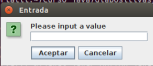
\includegraphics[scale=1]{imagenes/input.png}
\caption{InputDialog}
\end{figure}
\pause
 \begin{verbatim}
String inputValue = 
  JOptionPane.showInputDialog("Please input a value"); 
\end{verbatim}
\end{frame}

\subsection{Mensaje}
\begin{frame}[fragile]
    \frametitle{Mensaje}
Muestra un cuadro de diálogo al usuario, normalmente de carácter informativo
\begin{figure}
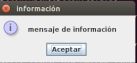
\includegraphics[scale=1]{imagenes/informacion.png}
\caption{showMessageDialog}
\end{figure}
\pause
 \begin{verbatim}
JOptionPane.showMessageDialog(null,
"mensaje de información",
"información", JOptionPane.INFORMATION_MESSAGE);
\end{verbatim}
\pause
Podemos emplear a parte de INFORMATION\_MESSAGE, QUESTION\_MESSAGE, WARNING\_MESSAGE o ERROR\_MESSAGE
\end{frame}


\section{Documentacion}
\begin{frame}[fragile]
Mejor consultar la documentacion de API javax.swing.JOptionPane de Oracle \vspace{1cm}
\pause
\begin{center}

\begin{Huge}
\textcolor{cyan}{FIN}
\end{Huge}
\end{center}
\end{frame}


\end{document}

